\documentclass[fontsize=12pt]{article}
%\usepackage{xeCJK}
\usepackage{amsfonts}
\usepackage{amssymb}
\usepackage{amsmath}
\usepackage{amsthm}
\usepackage{mathrsfs}
\usepackage{relsize}
\usepackage{bm}
\usepackage[dvipdfmx]{graphicx}
\theoremstyle{definition}
\newtheorem{definition}{Definition}
\newtheorem{theorem}{Theorem}[section]
%\setCJKmainfont{SimSun}
\title{Formula to Calculate Weight for Low-Weight Weight 3 Inputs and Proof} 
\author{Kwame Ackah Bohulu}
\date{\today}
\begin{document}
\maketitle

\newpage


\section{Equation and Proof}


\begin{theorem}
Let $Q(x) =x^{a\tau+t}(1+x^{\beta \tau +1}+x^{\gamma \tau +2})$ be the polynomial representation of a weight $3$ RTZ input.
The Hamming weight, $w_H$ of a turbo codeword generated by a weight-$3$ RTZ input is given by 
\begin{equation}
7+2(\max\{l_1,l_2\}+\max\{l^{\prime}_1,l^{\prime}_2\})
\end{equation}
\end{theorem}

\begin{figure}[h]
  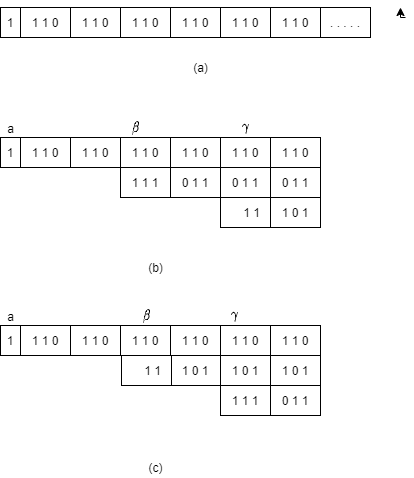
\includegraphics[scale=1,bb=0 0 30 30]{wt3_proof}
\caption{weigt-$3$ RTZ input Hamming weight equation proof}
\end{figure}

\begin{proof}
We know that the impule response of the RSC encoder is given by $\{1 1 1 0 1 1 0 1 1 0 1 1 0...\}$ with a cycle of $1 1 0$. We group the cycles into blocks as shown in Figure 1 (a)  and refer to each block as a layer, with the numbering of the layer beginning at $0$. If we assume that the weight-$3$ RTZ begins at the head of the weight-$3$ RTZ input, then $\beta$ and $\gamma$ can occur at either the 1st or second position within a layer. %Let $\mathcal{L}(\beta),\mathcal{L}(\gamma)$ represent the layer within which $\beta$ and $\gamma$ occur. If $\beta$ occupies the 1st position within a layer and $\gamma$ occupies the 2nd position within a layer, then $l_1 = \mathcal{L}(\beta)$ and $l_2 = \mathcal{L}(\gamma)$ and vice-versa.

Let the weight of the parity bit sequence be denoted by $w_p$. Calculating $w_p$ for the weight-$3$ RTZ requires 2 steps calculating the weight from $a$ to $\beta$ (denoted $w_{\Delta \beta}$) and the weight from $\beta$ to $\gamma$ denoted (denoted $w_{\Delta \gamma}$) . This is done for 2 cases

\paragraph {case 1. $\beta$ occupies the first position in its layer and $\gamma$, the second position (Figure 1(b))\newline}
let $l_1$ be the layer that $\beta$ is located in and $l_2$ be the layer that $\gamma$ is located in with reference to $a$.
To calculate $w_{\Delta \beta}$ we need to observe that each individual non-overlaping layer adds a weight of $2$ to $w_{\Delta \beta}$ whiles the fixed point adds weight $1$ to it. This means

$$w_{\Delta \beta} = 2l_1+1$$

To calculate $w_{\Delta \gamma}$, observe that each double-overlapping layers and the last layer each contribute  a weight of $2$ to $w_{\Delta \gamma}$ whiles $l_1$ adds a weight of 1. Therefore

$$w_{\Delta \gamma} = 2(l_2-l_1)+1$$

And 
\begin{equation}
\begin{split}
w_p&=2l_1+1 + 2(l_2-l_1)+1\\
&=2l_2+2
\end{split}
\end{equation}

\paragraph {case 2. $\beta$ occupies the second position in its layer and $\gamma$, the first position Figure 1(c) \newline}
let $l_1$ be the layer that $\beta$ is located in and $l_2$ be the layer that $\gamma$ is located in with reference to $a$.

To calculate $w_{\Delta \beta}$ we need to observe that each individual non-overlaping layer adds a weight of $2$ to $w_{\Delta \beta}$ whiles the fixed point and $l_1$ adds weight $1$ to it. This means

$$w_{\Delta \beta} = 2l_1+2$$

To calculate $w_{\Delta \gamma}$, observe that each double-overlapping layer contributes  a weight of $2$ to $w_{\Delta \gamma}$ whiles $l_1$ and $l_2$ each adds a weight of 1. Therefore

$$w_{\Delta \gamma} = 2(l_2-l_1)+2$$

And 
\begin{equation}
\begin{split}
w_p&=2l_1+1 + 2(l_2-l_1)+1\\
&=2l_2+2
\end{split}
\end{equation}

Making $\beta > \gamma$ and maintaining the definitions for $l_1$ and $l_2$, we get

$$w_p=2l_1+2$$
For both cases listed above.
We can see that, $w_p$ depends on wether $l_1$ or $l_2$ is furtherst from $a$, therefore
\begin{equation}
w_p=2(\max \{l_1,l_2\})+2
\end{equation}

Assuming that after interleaving $Q(x)$
 another weight-$3$ RTZ input 
  $Q'(x) =x^{a'\tau+t}(1+x^{\beta' \tau +1}+x^{\gamma' \tau +2})$is produced. Let $l'_1,l'_2$ be similarly defined  like $l_1$ and $l_2$. Then $w_H$ of the turbo codeword is given by
\begin{equation}
\begin{split}
w_H&=2(\max \{l_1,l_2\})+2+2(\max \{l'_1,l'_2\})+2+3\\
&=7+2(\max\{l_1,l_2\}+\max\{l^{\prime}_1,l^{\prime}_2\})
\end{split}
\end{equation}
\end{proof}

\end{document}
